%&latex
%
\providecommand{\main}{../..}
\documentclass[../../main.tex]{subfiles}

\begin{document}

\chapter{Variational methods}
Exactly solvable models are rare.\lesson{21}{27/04/20} For example, the Ising Model, describing in a very simplified manner a discrete set of local interacting binary variables, has been exactly solved only for $d=1$ in general, and for $d=2$ only in absence of an external field ($h=0$). The latter, in particular, requires long and sophisticated derivations.

Even for other models, the trend is the same: whenever we wish to study \textit{emergent phenomena} the problem usually becomes analytically intractable.

\medskip

One possibility is then to resort to \textbf{numerical simulations}. However, these are often time-consuming, require significant computational power, and can be hard to interpret - as interesting \q{high level} characteristics (such as the conditions for phase transitions) are drowned in lots of irrelevant \q{low-level} data. 

\medskip

So we may resort to \textbf{approximate computations} instead. The idea is to find a simple model that is able to capture, at least \textit{qualitatively}, features from a more complex one, while still admitting an exact solution. This can then give hints on \textit{what to look for} in a full numerical simulation, thus allowing a deeper understanding. 

\medskip

One quick way to compute approximations is through \textbf{variational methods}. In essence, we consider some parametrized pdf $f_{\bm{\theta}}(\bm{x})$, and tweak the parameters $\bm{\bm{\theta}}$ so that it becomes \q{closer and closer} to the target pdf $f(\bm{x})$ of the full model. If we choose a sufficiently \textit{simple} form for $f_{\bm{\theta}}$, we will be able to perform exact computations, while still retaining some sort of \q{correspondance} with the more complex model.

\medskip

In the following, we will first introduce a notion of \q{\textbf{distance}} between pdf\textit{s} (\textbf{relative entropy}), giving a mathematical meaning to the notion of \q{closeness} between probability distributions. Then we will explicitly state the \textit{variational method} as a \textbf{minimization problem}, and, using the Ising Model as an example, we will see a popular choice for the parametrization of $f_{\bm{\theta}}$: the \textbf{mean-field approximation}.  

\subsection{Relative Entropy}
Given two (discrete) probability distributions $\{p_i\}_{i \in \mathcal{D}}$ and $\{q_i\}_{i \in \mathcal{D}}$, with $p_i, q_i > 0$ and $\sum_i p_i = \sum_i q_i = 1$, we define the \textbf{relative entropy} (or Kullback–Leibler divergence) of $\{p_i\}$ with respect to $\{q_i\}$ as follows:
\begin{align}
    S_R(\{p_i\}, \{q_i\}) = -\sum_{i \in \mathcal{D}} p_i \ln \frac{p_i}{q_i} \leq 0 \label{eqn:relative-entropy}
\end{align}  
In a sense, relative entropy measures the \textit{closeness} between the two distributions - as it is maximum ($S_R=0$) when the two coincide, i.e. $p_i = q_i$ $\forall i$. Note, however, that $S_R$ is not a \textit{distance function} in the proper sense, as it does not satisfy the triangular inequality. 

\medskip

The fact that $S_R=0$ is the maximum point of $S_R$,\marginpar{Proof that $S_R \leq 0$} i.e. $S_R \leq 0$, can be proven as follows. First we define an auxiliary function $f(x)$ over $(0,\infty)$:
\begin{align*}
    f(x) = -x \ln x \qquad x > 0
\end{align*}
Such function $f(x)$ is \textbf{concave}. In fact: 
\begin{align*}
    f'(x) &= -1 - \ln x\\
    f''(x) &= -\frac{1}{x}  < 0 \qquad x > 0
\end{align*}
So, we may apply Jensen's inequality. For any choice of a set of non-negative numbers $\{\lambda_i\}$ summing to $1$, the following relation holds: %TO DO Add reference to 15/04 lecture (after adding ex. 5.17 and verification of Shannon Entropy's 3 defining properties)
\begin{align*}
    f\left(\sum_i \lambda_i x_i\right) \geq \sum_i f(x_i) \lambda_i \qquad \sum_i \lambda_i = 1 \> \land \> \lambda_i \geq 0
\end{align*}
And letting $\lambda_i = q_i$ and $x_i = p_i / q_i$ completes the proof:
\begin{align*}
    S_R = \sum_i q_i f\left(\frac{p_i}{q_i} \right) \leq f\left(\sum_i \bcancel{q_i} \frac{p_i}{\bcancel{q_i}} \right) = f(1) = 0
\end{align*}
with the equality holding if and only if $p_i = q_i$.

\subsection{Approximation as an optimization problem}
Let's consider, for simplicity, a system with \textbf{discrete} states $\{\bm{\sigma_i}\}_{i \in \mathcal{D}}$, each with energy $\mathcal{H}(\bm{\sigma_i})$, and an associated probability $q_i$ given by a Boltzmann distribution:
\begin{align*}
    \rho(\bm{\sigma_i}) \equiv q_i = \frac{e^{-\beta \mathcal{H}(\bm{\sigma_i})}}{Z} = e^{-\beta(\mathcal{H}(\bm{\sigma})-F)} \qquad Z = \sum_{\{\bm{\sigma}\}} e^{-\beta \mathcal{H}(\bm{\sigma})}\equiv e^{-\beta F}
\end{align*}
where $F$ is the system's \textbf{free energy} function.

\medskip

In general, the $\{q_i\}$ are difficult to explicitly compute, because $Z$ is generally a sum over a huge number of terms ($2^V$ in the case of the Ising Model) with no analytical form.

\medskip

So, the idea is to approximate $\rho$ with another \q{easier} distribution $\rho_0$, the \textbf{variational ansatz}, which is parametrized as a Boltzmann distribution with a different Hamiltonian $\mathcal{H}_0$ (and so also a different free energy $F_0$):
\begin{align}\label{eqn:variational-ansatz}
    \rho_0(\bm{\sigma_i}) \equiv p_i = \frac{e^{-\beta \mathcal{H}_0(\bm{\sigma_i})}}{Z_0} = e^{-\beta(\mathcal{H}_0(\bm{\sigma})-F_0)} \qquad Z_0 = \sum_{\{\bm{\sigma}\}} e^{-\beta \mathcal{H}_0(\bm{\sigma})} \equiv e^{-\beta F_0}
\end{align}

The \textit{closeness} of $\{p_i\}$ to $\{q_i\}$ is given by their \textbf{relative entropy} (\ref{eqn:relative-entropy}):
\begin{align} \nonumber
    0 \leq \sum_i p_i \ln \frac{p_i}{q_i} &= \sum_{\{\bm{\sigma}\}} \frac{e^{-\beta \mathcal{H}_0 (\bm{\sigma})}}{Z_0} \ln \frac{e^{-\beta \mathcal{H}_0(\bm{\sigma}) }}{\underbrace{Z_0}_{e^{-\beta F_0}} } \frac{\overbrace{Z}^{e^{-\beta F}} }{e^{-\beta \mathcal{H}(\bm{\sigma})}}  = \\
    &=  \nonumber
    \frac{1}{Z_0} \sum_{\{\bm{\sigma}\}} e^{-\beta H_0(\bm{\sigma})} \beta[\mathcal{H}(\bm{\sigma}) - \mathcal{H}_0(\bm{\sigma}) - F + F_0] =\\
    &= \beta \langle \mathcal{H}-\mathcal{H}_0 \rangle_0 - \beta (F-F_0) \label{eqn:rel-entr}
\end{align} 
where $\langle \cdots \rangle_0$ denotes the average according to the ansatz distribution:
\begin{align*}
    \langle f(\bm{\sigma}) \rangle_0 \equiv \frac{1}{Z_0} \sum_{\{\bm{\sigma}\}} e^{-\beta \mathcal{H}_0(\sigma)} f(\bm{\sigma})
\end{align*}
The expression (\ref{eqn:rel-entr}) is called the \textbf{Gibbs-Bogoliubov-Feynman inequality}\footnote{Physically, it is completely equivalent to the second law of thermodynamics.}, and holds as an equality if and only if $\rho = \rho_0 \Leftrightarrow \mathcal{H} = \mathcal{H}_0$. 

\medskip

Rearranging (\ref{eqn:rel-entr}):
\begin{align}\label{eqn:ineq-1}
    \beta F \leq \beta F_0 + \beta \langle \mathcal{H} - \mathcal{H}_0 \rangle_0 = \beta \langle \mathcal{H} \rangle_0 + \beta {(F_0 - \langle \mathcal{H}_0 \rangle_0)}
\end{align}
Note that $F_0$ does not depend on $\bm{\sigma}$, as it's $\propto \ln Z_0$, and so we can bring it inside the average, and expand it:
\begin{align*}
    \beta (F_0 - \langle \mathcal{H}_0 \rangle_0) = \beta \langle F_0 - \mathcal{H}_0 \rangle_0 =  \sum_{\{\bm{\sigma}\}} \rho_0(\bm{\sigma}) \hlc{Yellow}{\beta(F_0 - \mathcal{H}_0(\bm{\sigma}))}
\end{align*}
Then, from (\ref{eqn:variational-ansatz}) note that:
\begin{align*}
    \rho_0(\bm{\sigma}) = e^{-\beta (\mathcal{H}_0(\bm{\sigma}) - F_0)} \Rightarrow \hlc{Yellow}{\ln \rho_0(\bm{\sigma})} = \beta(F_0 - \mathcal{H}_0(\bm{\sigma}))
\end{align*}
and substituting above:
\begin{align}\label{eqn:s-entropy}
    \beta (F_0 - \langle \mathcal{H}_0 \rangle_0) =\textcolor{Red}{-}\frac{1}{\textcolor{Red}{k_B}}\underbrace{\Big( \textcolor{Red}{-k_B} \sum_{\{\bm{\sigma}\}} \rho_0(\bm{\sigma}) \ln \rho_0(\bm{\sigma})\Big)}_{S[\rho_0]}  = -\frac{S[\rho_0]}{k_B} 
\end{align}
where $S[\rho_0]$ is the \textbf{information entropy} of $\rho_0$:
\begin{align*}
    S[\rho_0] = -k_B \sum_{\{\bm{\sigma}\}} \rho_0(\bm{\sigma}) \ln \rho_0(\bm{\sigma})
\end{align*} 

Thus, substituting (\ref{eqn:s-entropy}) back in the inequality (\ref{eqn:ineq-1}) leads to:
\begin{align}\label{eqn:var-principle}
    \beta F \leq  \beta \langle \mathcal{H} \rangle_0 -\frac{S[\rho_0]}{k_B} = \beta \langle \mathcal{H} \rangle_0 - {\beta T S[\rho_0]}
\end{align}
And dividing by $\beta$:
\begin{align*}
    F \leq F_V \equiv \langle \mathcal{H} \rangle_0 - T S[\rho_0]
\end{align*}
where $F_V$ is called the \textbf{Variational Free Energy} (VFE). 

So,  the true free energy $F$ is always less or equal to the variational one $F_V$. An optimal estimate of $F$ is obtained by minimizing $F_V$ with respect to $\rho_0$.

\medskip

Clearly, if we do not require any constraint on $\rho_0$, thus allowing arbitrary complexity, then the minimum is obtained when $\rho_0 = \rho$: the most accurate approximation of a model is the model itself. Realistically $\rho$ is mathematically intractable, and we need to \textit{bound} the \q{complexity} of $\rho_0$, with the effect that it won't be able to perfectly replicate $\rho$, and so the minimum for $F_V$ will be larger than $F$ (but hopefully still somewhat close).

\medskip

One possible way to constrain the \q{complexity} of $\rho_0$ is to \textit{force it} to be separable: 
\begin{align}\label{eqn:mean-field}
    \rho_0(\bm{\sigma}) = \prod_x \rho_x (\sigma_x)
\end{align} 
In this way, all degrees of freedom of the system become \textbf{decoupled}. In a sense, correlations and complex behaviours are \q{averaged} between each component - and in fact the approximation in (\ref{eqn:mean-field}) is known as the \textbf{mean field} ansatz. 

\section{Mean Field Ising Model}
Consider a $d$-dimensional nearest-neighbour Ising Model, where we allow each spin to interact with a \textbf{local} magnetic field $b_x$, leading to the Hamiltonian:
\begin{align*}
    \mathcal{H}(\bm{\sigma}) = -J \sum_{\langle x,y \rangle} \sigma_x \sigma_y - \sum_x b_x \sigma_x
\end{align*}
To understand its behaviour, we use the \textbf{mean-field} approximation (\ref{eqn:mean-field}), and choose a parametrization inspired by the non-interacting Ising Model (\ref{eqn:rho1-m}, pag. \pageref{eqn:rho1-m}):
\begin{align} \label{eqn:mfi}
    \rho_0(\bm{\sigma}) = \prod_x \rho_x(\sigma_x) \qquad \rho_x(\sigma_x) = \frac{1+\textcolor{Blue}{m_x} \sigma_x}{2} \quad m_x \in [-1,1]
\end{align}
where the $\{m_x\}$ are the \textit{variational parameters} that will be \textit{tweaked} to make $\rho_0(\bm{\sigma})$ closer to the real probability distribution $\rho(\bm{\sigma})$ of the Ising Model, by minimizing the \textbf{variational free energy} $F_V$. The constraint $m_x \in [-1,1]$ comes from requiring all probabilities to be non-negative $\rho_x(\sigma_x) \geq 0$.

Before proceeding, note that (\ref{eqn:mfi}) is already normalized:
\begin{align*}
    \sum_{\sigma_x = \pm 1}\rho_x(\sigma_x) = \frac{1+m_x}{2} + \frac{1-m_x}{2} = \frac{1}{2} + \frac{1}{2} = 1    
\end{align*}

and that each \textit{variational parameter} $m_x$ corresponds to the \textbf{local magnetization} of spin $\sigma_x$ \textit{in the mean-field model}: 
\begin{align}\nonumber
    \langle \sigma_x \rangle_0 &= \sum_{\{\bm{\sigma}\}} \rho_0(\bm{\sigma}) \sigma_x = \sum_{\{\bm{\sigma}\}} \prod_y \frac{1+m_y \sigma_y}{2} \sigma_x =  \\ \nonumber
    &\underset{(a)}{=}  \sum_{\sigma_x = \pm 1} \Bigg(\prod_{y \neq x} \underbrace{\sum_{\sigma_y = \pm 1} \frac{1+m_y \sigma_y}{2}}_{1} \Bigg) \frac{1+m_x \sigma_x}{2} \sigma_x =\\ 
    &=
    \sum_{\sigma_x = \pm 1} \sigma_x \frac{1+m_x \sigma_x}{2} = \frac{1+m_x}{2} - \frac{1-m_x}{2} =  m_x \label{eqn:local-average}
\end{align}
where in (a) we split the product in the case $y \neq x$ and $y = x$. Also note that the average is over $\rho_0$ and not the \q{true} pdf $\rho$.

\begin{expl}\textbf{Choice of parametrization}.  
    The distribution $\rho_x(\sigma_x)$ in (\ref{eqn:mfi}) is the most general discrete distribution for a binary variable such as $\sigma_x$, just rewritten to highlight the average $m_x$.

    In fact, consider a generic \textbf{binary} variable $\sigma$. Its distribution is:
    \begin{align*}
        \mathbb{P}[\sigma = +1] = p_+ \qquad \mathbb{P}[\sigma=-1] = p_-
    \end{align*}
    Due to normalization, $p_+ + p_- = 1$, and so there is only \textbf{one free parameter} needed to completely specify the pdf:
    \begin{align*}
        \mathbb{P}[\sigma = +1] = p \qquad \mathbb{P}[\sigma = -1] = 1-p
    \end{align*}  
    
    If we then rewrite $p$ as function of the average $\langle \sigma \rangle = m$, we get:
    \begin{align*}
        m = \sum_{\sigma = \pm 1} \sigma\mathbb{P}[\sigma] = p - (1-p) = 2p + 1 \Rightarrow p = \frac{1+m}{2} 
    \end{align*}
    And so:
    \begin{align*}
        \mathbb{P}[\sigma = +1] = \frac{1+m}{2} \qquad \mathbb{P}[\sigma = -1] = \frac{1-m}{2}  
    \end{align*}
    Which can be rewritten more compactly as:
    \begin{align*}
        \rho(\sigma) = \frac{1+m \sigma}{2} 
    \end{align*}
    So we are not making any additional hypothesis other than that of a separable $\rho(\bm{\sigma})$ (given by the mean field approximation).
\end{expl}


For simplicity, we work with $\beta F_V$, denoting $\beta J \equiv K$ and $\beta b_x \equiv h_x$. From the variational principle (\ref{eqn:var-principle}):
\begin{align}
    \beta F \leq  
    \min_{\bm{m}} \beta F_V(\bm{m}, \bm{h}) = \min_{\bm{m}} \left(
      \beta \langle \mathcal{H} \rangle_0 -\frac{S[\rho_0]}{k_B} \right) 
      \label{eqn:ising-variational}
\end{align}
The average of $\mathcal{H}$ according to the ansatz is:
\begin{align*}
    \langle \mathcal{H} \rangle_0 = \langle -J \sum_{\langle x,y \rangle} \sigma_x \sigma_y - \sum_x b_x \sigma_x \rangle_0 = -J \sum_{\langle x,y \rangle} \langle \sigma_x \sigma_y \rangle_0 - \sum_x b_x \langle \sigma_x \rangle_0
\end{align*}
We already computed $\langle \sigma_x \rangle_0 = m_x$ in (\ref{eqn:local-average}). For the two-point correlation, as $\rho_0$ is separable and thus $\sigma_x$ and $\sigma_y$ are decoupled, we get:
\begin{align*}
    \langle \sigma_x \sigma_y \rangle_0 = \langle \sigma_x \rangle_0 \langle \sigma_y \rangle_0 = \sum_{\sigma_x} \frac{1+m_x \sigma_x}{2} \sigma_x \sum_{\sigma_y} \frac{1+m_y \sigma_y}{2} \sigma_y = m_x m_y
\end{align*}
Thus:
\begin{align}\label{eqn:H0avg}
    \langle \mathcal{H}(\bm{\sigma}) \rangle_0 = -J \sum_{\langle x,y \rangle} m_x m_y - \sum_x b_x m_x = \mathcal{H}(\bm{m})
\end{align}
This is valid more in general when applying the mean field approximation to even more complex Hamiltonians, as it is a consequence of the separability of $\rho_0$.

\medskip

On the other hand, the entropy of $\rho_0$ can be directly computed. Noting that $\rho_x(\sigma_x)$ is exactly the same pdf we used in the non-interacting Ising Model, we can borrow the results (\ref{eqn:lstep}) and (\ref{eqn:lstepb}, pag. \pageref{eqn:lstep}) from there:
\begin{align}\nonumber
    -\frac{S[\rho_0]}{k_B} &= \sum_{\{\bm{\sigma}\}} \rho_0(\bm{\sigma}) \ln \rho_0(\bm{\sigma}) = \sum_x \sum_{\sigma_x} \frac{1+m_x \sigma_x}{2} \ln \frac{1+m_x \sigma_x}{2} =\\ \label{eqn:rho0-ent}
    &= \sum_x \left(\frac{1+m_x}{2} \ln \frac{1+m_x}{2} + \frac{1-m_x}{2} \ln \frac{1-m_x}{2} \right)  \equiv \sum_x s_0(m_x)
\end{align}
where we defined a \textit{local entropy} $s_0$ as: 
\begin{align*}
    s_0(m) \equiv \frac{1+m}{2} \ln \frac{1+m}{2} + \frac{1-m}{2} \ln \frac{1-m}{2}    
\end{align*}
Substituting these results (\ref{eqn:H0avg}) and (\ref{eqn:rho0-ent}) back in (\ref{eqn:ising-variational}) we arrive to:
\begin{align} \label{eqn:var-free-energy}
    \beta F_V(\bm{m}, \bm{h}) &= \beta H(\bm{m}) + \sum_x s_0(m_x) =\\
    &= -K \sum_{\langle x,y \rangle} m_x m_y - \sum_x h_x m_x + \sum_x \left[\frac{1+m_x}{2} \ln \frac{1+m_x}{2} + \frac{1-m_x}{2} \ln \frac{1-m_x}{2}    \right] \nonumber
\end{align}
where the first line holds for a generic Hamiltonian $\mathcal{H}(\bm{\sigma})$, and the second is specific for the Ising Model we are studying.

\medskip

Then, we minimize $F_V(\bm{m}, \bm{h})$ with respect to $\bm{m}$, denoting the minimum as $F_V(\bm{M}, \bm{h})$:
\begin{align}
    \label{eqn:minimize}
    \pdv{m_x} \beta F_V \Big|_{\bm{m} = \bm{M}} \overset{!}{=}  0 \span \\ \nonumber
    0 &\overset{!}{=} \pdv{m_x} \left[-K \sum_{\langle x,y \rangle} m_x m_y - \sum_x h_x m_x + \sum_x \left(\frac{1+m_x}{2} \ln \frac{1+m_x}{2} + \frac{1-m_x}{2} \ln \frac{1-m_x}{2}    \right) \right]_{\quad\mathclap{\bm{m} = \bm{M}}} =\\ \nonumber
    &=-K\sum_{y \in \langle x,y \rangle} M_y - h_x + \frac{1}{2}\ln \frac{1+M_x}{2} + \cancel{\frac{1+M_x}{2} \frac{2}{1+M_x}\frac{1}{2}} - \frac{1}{2} \ln \frac{1-M_x}{2} - \cancel{\frac{1-M_x}{2} \frac{2}{1-M_x}\frac{1}{2}} =\\ \nonumber
    &= -K\sum_{y \in \langle x,y \rangle} M_y -h_x + \frac{1}{2} \ln\left(\frac{1+M_x}{\cancel{2}} \frac{\cancel{2}}{1-M_x}  \right) 
\end{align} 
where the sum is over all nodes $y$ neighbouring $x$, i.e. the ones included in some pair of neighbours $\langle y,x \rangle$ involving $x$.

Using the identity (\ref{eqn:inv_tanh}, pag. \pageref{eqn:inv_tanh})
\begin{align*}
    \tanh^{-1} M_x = \frac{1}{2} \ln \frac{1+M_x}{1-M_x}  
\end{align*}
and rearranging leads to:
\begin{align}\label{eqn:variational-sol}
    M_x(\bm{h}, K) = \tanh \left[K \sum_{y \in \langle y, x\rangle} M_y + h_x\right]
\end{align}

\subsection{Physical meaning of the variational parameters $M_x$}

It would be interesting to associate some physical meaning to the variational solution, and in particular understand what the $M_x$ represent. 

\medskip

So, we found that:
\begin{align*}
    \min_{\bm{m}} F_V(\bm{m}, \bm{h}) \equiv F_V(\bm{M}, \bm{h})
\end{align*}
with the $\bm{M}$ given by solving the $N$ equations (\ref{eqn:variational-sol}), one for each node. 

\medskip

The \textit{magnetization} given by the variational free energy is:
\begin{align} \nonumber
    \langle \sigma_x \rangle_V &\underset{\mathclap{(\ref{eqn:magnetization})}}{=} -\pdv{h_x} [\beta F_V(\bm{M}, \bm{h})] = -\beta \Bigg[\underbrace{\sum_y {\pdv{F_V}{m_y}}(\bm{m}, \bm{h})}_{0\> (\ref{eqn:minimize})} \pdv{m_y}{h_x} - \underbrace{{\pdv{F_V}{h_x}}(\bm{m}, \bm{h})}_{M_x \> (\ref{eqn:var-free-energy})}\Bigg]_{\bm{m} = \bm{M}} =\\
    &= M_x \label{eqn:MX-meaning}
\end{align} 
Note that the variational free energy $F_V$ \textbf{is not} the \textit{ansatz free energy} $F_0$, and so $\langle \sigma_x \rangle_V$ and $\langle \sigma_x \rangle_0$ are different averages, and (\ref{eqn:MX-meaning}) should not be confused with (\ref{eqn:local-average}). 

\medskip

So, $M_X$ is the best estimate of the \textit{true magnetization} $\sigma_x$, as it is obtained with the $F_V$ \textit{closest} to the real $F$.

\subsection{Uniform case}
Suppose the magnetic field is uniform $h_x \equiv h$. In this case, the system is \textbf{translationally invariant}. So, it is reasonable to consider the \textit{ansatz} where also all the local magnetizations are the same: $m_x \equiv m$, and search for a single value of $m$.

\medskip

Given these assumptions, (\ref{eqn:var-free-energy}) becomes:
\begin{align*}
    \beta F_V(m, h) &= -K m^2 \sum_{\langle x,y \rangle} 1 - mh\sum_x1 + \left[\frac{1+m}{2} \ln \frac{1+m}{2} + \frac{1-m}{2} \ln \frac{1-m}{2} \right] \sum_x 1 
\end{align*}
Then $\sum_x 1$ is just the number of nodes $N$, and $\sum_{\langle x,y \rangle} 1$ is the number of possible pairs, which is $N d$ for a $d$-dimensional cubic lattice (each node contributes with one pair for every possible \textit{direction}). Dividing by $N$:
\begin{align}\label{eqn:FV-uniform}
    \beta \frac{F_V(m,K,h)}{N} = - K d m^2 + \frac{1+m}{2} \ln \frac{1+m}{2} + \frac{1-m}{2} \ln \frac{1-m}{2} - hm   
\end{align}

The equation for $M_X$ (\ref{eqn:variational-sol}) becomes:
\begin{align*}
    M(h, K) = \tanh \left[KM \sum_{y \in \langle y, x\rangle} 1 + h\right]
\end{align*}
The sum is over all \textit{neighbours} of $x$, which are $2d$ for a $d$-dimensional cubic lattice ($2$ for every \textit{direction}), leading to:
\begin{align}
    \label{eqn:uniform-variational-eq}
    M(h,K) = \tanh(2dKM + h)
\end{align} 

\subsubsection{A. No external field}
Let's start with the case of no external field $h=0$. \marginpar{Case 1. $h=0$}
In this case, the variational free energy (\ref{eqn:FV-uniform}) is an \textbf{even}  function of $m$: 
\begin{align*}
    F_V(m,0) = F_V(-m,0)
\end{align*}
We can then study the solutions of (\ref{eqn:uniform-variational-eq}):
\begin{align}\label{eqn:h0case}
    \textcolor{Blue}{M} = \tanh(2dK\textcolor{Blue}{M}) \qquad M(K,0) \equiv M(K)
\end{align}
Clearly $M=0$ is always a solution. Depending on $2dK$, there can be two more solutions, as can be seen by plotting each side and looking for intersections (\ref{fig:uniformh0}).

\begin{figure}[H]
    \centering
    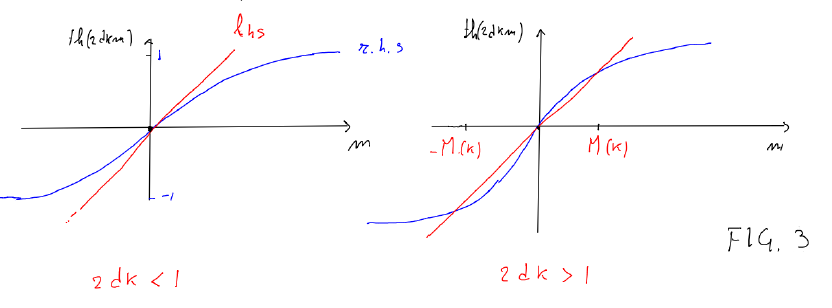
\includegraphics[width=0.9\textwidth]{uniformh0.png}
    \caption{Solutions of (\ref{eqn:uniform-variational-eq}) are intersections of the two curves.}
    \label{fig:uniformh0}
\end{figure}

The plots in (\ref{fig:uniformh0}) can be obtained by expanding $\tanh x$ in Taylor series around $x = 0$. The first three derivatives are:
\begin{align*}
    \dv{x} \tanh x &= 1- \tanh^2 x\\
    \dv[2]{x} \tanh x &= -2 \tanh x(1-\tanh^2 x)\\
    \dv[3]{x} \tanh x &= -2(1-\tanh^2 x ) + 4\tanh^2 x (1-\tanh^2 x)
\end{align*}
So:
\begin{align}\nonumber
    \tanh x &= \tanh 0 +x \dv{x}\tanh x\Big|_{x=0} + \frac{x^2}{2} \dv[2]{x} \tanh x\Big|_{x=0} + \frac{x^3}{3!}\dv[3]{x} \tanh x\Big|_{x=0} + \dots = \\
    &= x -\frac{2x^3}{3\cdot 2 \cdot 1} + O(x^5) = x -\frac{x^3}{3} + O(x^5) 
    \label{eqn:tanh-exp}
\end{align}
For small $x$, $\tanh x$ is linear, and in particular $\tanh(2d K M)$ is a line passing through the origin with slope $2dK$. It that slope is \textbf{less}  than te one of $y=M$, i.e. $1$, then the only intersection is at $M=0$ (left of fig. \ref{fig:uniformh0}). However, if $2dK > 1$, then there will be two other solutions (right of fig. \ref{fig:uniformh0}). 

In summary:
\begin{itemize}
    \item $2dK < 1 \Rightarrow K < K_c \equiv 1/2d$, (\ref{eqn:h0case}) has only one solution $M=0$.
    \item If $2dK > 1 \Rightarrow K > K_c$, there are $3$ solutions: $M=0, \pm M(K)$.
\end{itemize}

In the case $K > K_c$, we need to understand which of the three solution leads to the absolute minimum of $F_V$. So, let's proceed by expanding $\beta F_V(m,0)/N \equiv f(m)$ (\ref{eqn:FV-uniform}) for small $m$. The first four coefficients are:
\begin{align*}
    f(0) &= \frac{1}{2} \ln \frac{1}{2} + \frac{1}{2} \ln \frac{1}{2} = -\frac{1}{2} \ln 2 - \frac{1}{2}\ln 2 = -\ln 2\\
    f'(0) &= -2 K d m + \cancel{\frac{1}{2}\ln \frac{1+m}{2}} + \bcancel{\frac{1}{2}} -\cancel{\frac{1}{2}\ln \frac{1-m}{2}} -\bcancel{\frac{1}{2}} \Big|_{m=0} = 0\\
    f''(0) &= -2Kd +\frac{1}{4}\frac{2}{1+m} +\frac{1}{4}\frac{2}{1-m}\Big|_{m=0} = 1-2Kd    \\
    f^{(3)}(0) &= -\frac{1}{2(1+m)^2} + \frac{1}{2(1-m)^2} \Big|_{m=0} = 0  \\
    f^{(4)}(0) &= -\frac{1}{2}\frac{-2}{(1+m)^3} + \frac{1}{2}(-2)\frac{-1}{(1-m)^3} \Big|_{m=0} = 2    
\end{align*}
Clearly all odd terms vanish because $F_V(m,0)$ is \textbf{even}. Then: 
\begin{align*}
    \frac{\beta F_V(m, h=0)}{N} &= f(0) + mf'(0) + \frac{m^2}{2}f''(0) + \frac{m^3}{3!}f^{(3)}(0) + \frac{m^4}{4!}f^{(4)}(0) + \dots =\\
    &= -\ln 2 +\hlc{Yellow}{\frac{1-2Kd}{2}} m^2  + \frac{m^4}{12} + O(m^6) 
\end{align*}
Let's focus on the highlighted quadratic term. We distinguish three cases:

\begin{enumerate}
    \item When $\textcolor{Blue}{2Kd < 1}$ ($K < K_c$) the coefficient its positive, meaning that, for $x \sim 0$, $F_V$ behaves like a convex parabola (left of fig. \ref{fig:variational_cases}). As $K = \beta J = J/k_B T$, this holds for $T > T_c = 2d J/k_B$, where $T_c$ is called the system's \textbf{critical temperature}. 

    Note how, in this case, the variational free energy has a single global minimum at $m=0$.
    \item Now, if we let $\textcolor{Blue}{2Kd = 1}$ ($K=K_c = 1/2d$, or $T=T_c = 2dJ/k_B$), then the quadratic coefficient vanishes, and for $m \sim 0$ the variational free energy has the shape of a \textit{quartic} ($m^4$), meaning that it is close to $0$ and \q{very flat} for $m \to 0$. Still, there is only one global minimum at $m=0$.
    \item However, if $\textcolor{Blue}{2Kd > 1}$, then $F_V$ is like a \textbf{concave} parabola near the origin. So $m=0$ becomes a local maximum, and $m = \pm M(K)$ are two equivalent local minima. 
\end{enumerate}

\begin{figure}[H]
    \centering
    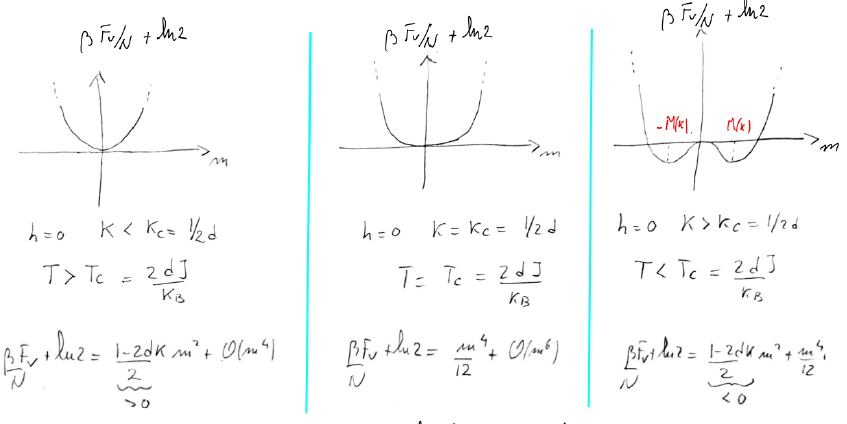
\includegraphics[width=0.9\textwidth]{variational_cases.png}
    \caption{} %TODO Add caption
    \label{fig:variational_cases}
\end{figure}

Thus, depending on the \textbf{temperature}, the system's behaviour changes \textit{fundamentally}.  

\medskip

Once we have found the solution $M$ for the minimum, the \textbf{best estimate} of the exact \textit{free energy} $\beta F$ is given by \ref{eqn:FV-uniform} evaluated at $m=M$ and $h=0$:
\begin{align*}
    \beta \frac{F_V(M,H,0)}{N} = -K d M + \frac{1+M}{2} \ln \frac{1+M}{2} + \frac{1-M}{2} \ln \frac{1-M}{2}     
\end{align*}

\subsubsection{Physical meaning of $M(K)$}
When $T < T_c$, we found\marginpar{$M(K)$ and the spontaneous magnetization} that the free energy is best approximated by a function with two local minima at $\pm M(K)$ - which we have interpreted as estimates of the system's \textbf{magnetization}. So, this mechanism could explain the experimentally observed phenomenon of \textbf{spontaneous magnetization}.

\medskip

Explicitly, we defined the spontaneous magnetization \textit{per node}  $m_S$ (\ref{eqn:break1}) as:
\begin{align}\label{eqn:ms}
    -\lim_{h \downarrow 0} \frac{1}{N} \lim_{N \uparrow \infty} \pdv{h} (\beta F) = \lim_{h \downarrow 0} \langle \frac{\sum_x \sigma_x}{N}  \rangle = m_S
\end{align}
In particular, the thermodynamic limit must be taken \textbf{before} the $h \to 0$ limit.

We can now use the variational free energy to compute an estimate of $m_S$. Note that in (\ref{eqn:FV-uniform}), the free energy density \textit{does not} depend on $N$, so the limit of $N \to \infty$ is trivial. Then we just need to differentiate with respect to $h$ and set $m = M$, the minimum found by solving (\ref{eqn:h0case}). Thus, the \textit{variational estimate} of $m_S$ is given by:
\begin{align}\nonumber
    m_S\Big|_{\mathrm{var.}} &= -\lim_{h \downarrow 0} \pdv{h} \frac{F_V(M, K, h)}{N} = -\lim_{h \downarrow 0} \Bigg[\underbrace{{\pdv{F_V}{m}}(m, K, h)}_{0\ (\ref{eqn:minimize})} \pdv{M}{h} + \underbrace{{\pdv{F_V}{h}}(m, K, h)}_{-m\ (\ref{eqn:FV-uniform})} \Bigg]_{\quad\mathclap{m = M}} \mathclap{=} \\
    &= \lim_{h \downarrow 0} M(K,h) = M(k)
    \label{eqn:variational-spontaneous-magnetization}
\end{align} 
where $M(K,h)$ is the solution of (\ref{eqn:uniform-variational-eq}), which, in the limit $h \to 0$, becomes one of the solutions we found in the $h=0$ case, since it is an analytic function. So $m_S = 0$ if $2dK < 1$, and $\neq 0$ otherwise.

\medskip

We can then study how the solution $M(K)$ of (\ref{eqn:h0case}) varies as a function of $K^{-1} = k_B T/J$. This can be done numerically - but to get some understanding we consider the case near criticality $K \approx K_c = 1/2d$. From fig. \ref{fig:uniformh0} and fig. \ref{fig:variational_cases} we expect $M \approx 0$ when $K \approx K_c$.

\medskip

So, using the expansion of $\tanh x$ (\ref{eqn:tanh-exp}) for small $x$, (\ref{eqn:h0case}) becomes:
\begin{align*}
    M = 2dKM- \frac{(2dK)^3 M^3}{3} + O(M^5) 
\end{align*}
One solution is clearly $M=0$, $\forall K$. 

For the other \textbf{solutions},\marginpar{$M(K)$ near criticality} we suppose that $K > K_c = 1/2d$, e.g. $K = K_c + \delta$ with $\delta \approx 0^+$, and then divide by $M$ to get:
\begin{align*}
    M^2 &= \frac{3}{(2dK)^3}(2dK-1) + O(M^4) =\\
        &= \frac{6d}{(K/K_c)^3} (K-K_c)  + O(M^4) =\\
        &= \frac{6d}{[(K_c + \delta)/K_c]^3} (\cancel{K_c}+\delta - \cancel{K_c}) + O(M^4) =\\
        &= 6d \frac{\delta}{(1+ \delta/K_c)^3} + O(M^4) =\\
        &= 6d \delta + O(\delta^2)
\end{align*}
For $\delta \approx 0$, $\delta/(1+ \delta/K_c)^3 \approx \delta$, and so $M^2$ is of order $\delta$, meaning that $M^4$ is of order $\delta^2$. 

Taking the square root:
\begin{align}\label{eqn:mean-field-MS}
    M(K) = \sqrt{6d} (K-K_c)^\beta + O(K-K_c)
\end{align}
where $\beta = 1/2$ is the \textbf{critical exponent}. Note that the behaviour of the spontaneous magnetization\marginpar{Critical exponent and universality} near criticality is given by a power law in the distance to the critical point $K_c$: this happens more in general, not only for the Ising Model, and does not depend on the details of the model  (\textbf{universality}). (\ref{eqn:mean-field-MS}) also produces a \textbf{singularity} at $K=K_c$, where $M(K)$ starts rising from $0$ in a non-smooth manner (fig. \ref{fig:MK_plot}).

\begin{figure}[H]
    \centering
    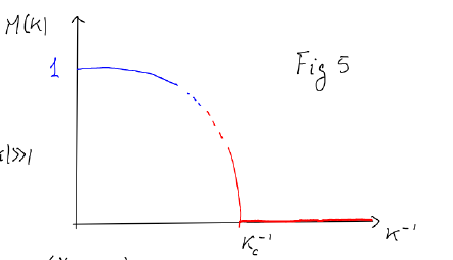
\includegraphics[width=0.7\textwidth]{MK_plot.png}
    \caption{Plot of the spontaneous magnetization $M(K)$ (estimated from the variational free energy) as function of temperature ($K^{-1} \propto T$).
    From fig. \ref{fig:variational_cases} we know that $M(K) = 0$ for $K < K_c$. The red curve at $K \approx K_c$ is given by (\ref{eqn:mean-field-MS}), while the blue curve at $K \to \infty$ derives from (\ref{eqn:low-temperature-var})
    Note the \textbf{singularity} at $K=K_c$, the critical point. }
    \label{fig:MK_plot}
\end{figure}

The result in (\ref{eqn:mean-field-MS})\marginpar{The validity of the mean field approximation} is an estimate given by the mean field approximation. However, the same kind of relation \textit{holds} in the true model, just with a different exponent $\beta$. For the $d=2$ case, $\beta = 1/8$ can be exactly determined, while for $d > 2$ one resorts to numerical methods, obtaining $\beta \approx 0.31$ at $d=3$, and - surprisingly - $\beta = 1/2$ for $d > 3$. Again, this is not a specific behaviour: the mean field approximation happens to become \textbf{exact} in $d \geq 4$ in many cases, as we will see later on.   

\medskip

If we instead study the behaviour at low temperatures ($K \gg 1$), we expect from fig. \ref{fig:uniformh0} to see $M \approx 1$, meaning that the argument $2dKM(k)$ of the tangent in (\ref{eqn:h0case}) becomes very large. So we expand $\tanh x$ accordingly:
\begin{align*}
    \tanh x &= \frac{e^x - e^{-x}}{e^x + e^{-x}} \frac{\textcolor{Red}{e^{-x}}}{\textcolor{Red}{e^{-x}}} = \frac{1-e^{-2x}}{1+e^{-2x}} \underset{(a)}{=}  (1-e^{-2x})(1-e^{-2x} + e^{-4x} + \dots) =\\
    &= 1 - 2e^{-2x} + 2e^{-4x} + O(e^{-6x})
\end{align*}
where in (a) we used the geometric series expansion:
\begin{align*}
    \frac{1}{1+x} = 1 - x + x^2 - x^3 + \dots
\end{align*}

And substituting in (\ref{eqn:h0case}) we get:
\begin{align}\label{eqn:low-temeperature-var}
    M(K) = 1-2e^{-4dK M(k)} + O(e^{-8KdM(k)}) \underset{(b)}{=}  1-2e^{-4dK} + O(e^{-12dK})
\end{align}
where in (b) we substituted $M(k) \approx 1$ in the right side, noticing that all other terms are of order $e^{-12dK}$ or higher. This result agrees with the low temperature expansion we did in the $d=2$ case in (\ref{eqn:m-low}, pag. \pageref{eqn:m-low}). So the spontaneous magnetization quickly approaches $1$ when $K^{-1} \to 0$ ($T \to 0$).

\subsubsection{B. External field}
If $h\neq 0$, from (\ref{eqn:FV-uniform}) we have:\marginpar{2. Case $h\neq 0$}
\begin{align*}
    \beta \frac{F_V(m, K, h)}{N} = \beta \frac{F_V(m,K,0)}{N} - hm  
\end{align*}
So the variational equations (\ref{eqn:minimize}) become:
\begin{align}\label{eqn:var-eq-h}
    h &= \pdv{m}\left[\beta \frac{F_V(m,K,0)}{N} \right]_{m=M} = (\tanh^{-1} m - 2dKm)\Big|_{m=M} =\\
      &\underset{\mathclap{M \approx 0}}{=}  M(1-2dK) + \frac{M^3}{3} + \frac{M^5}{5} + \frac{M^7}{7} + \dots \nonumber
\end{align}
Depending on the sign of $1-2dK$, i.e. if $2dK$ is lower of higher than $1$, the slope at the origin will be either positive or negative, leading to the plots in fig. \ref{fig:hplot}.

\begin{figure}[H]
    \centering
    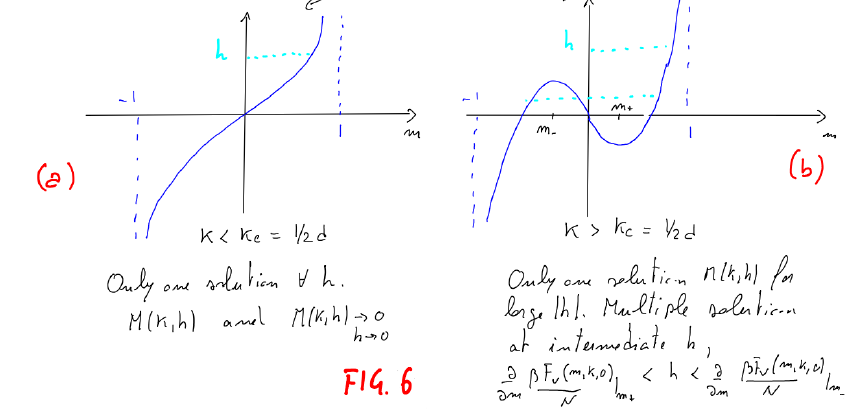
\includegraphics[width=0.9\textwidth]{hplot.png}
    \caption{Plot of the right hand side of (\ref{eqn:var-eq-h}), i.e. the variational estimate of magnetization,
as function of $m$.} %TODO Caption
    \label{fig:hplot}
\end{figure}

So there are two cases:
\begin{enumerate}
    \item If $K < K_c = 1/2d$, then the right side of (\ref{eqn:var-eq-h}) is strictly increasing, and so admits only one intersection with an horizontal line $y = h$, meaning that there is only one solution for $M(h,K)$ (in general $\neq 0$). If we then let $h \to 0$, $M(K,h) \to 0$ smoothly, and so $m_S = 0$, as expected. 
    \item If $K > K_c$, instead, the plot is the one on the right of fig. \ref{fig:hplot}, and multiple intersections with $y=h$ are possible if $h$ lies in a certain range:
    \begin{align*}
        \pdv{m} \frac{\beta F_V(m,K,0)}{N} \Big|_
        {m_+} < h < \pdv{m} \frac{\beta F_V(m,K,0) }{N}\Big|_{m_-}
    \end{align*}
    where $m_\pm$ are the local minima/maxima of the right side of (\ref{eqn:var-eq-h}).
\end{enumerate}

In the $K>K_c$ case, in order to understand which of the possible multiple solutions $\{M_i\}_{i=1,2,3}$ corresponds to the minimum of $F_V$ we refer to fig. \ref{fig:variational_energy_h}.

\begin{figure}[H]
    \centering
    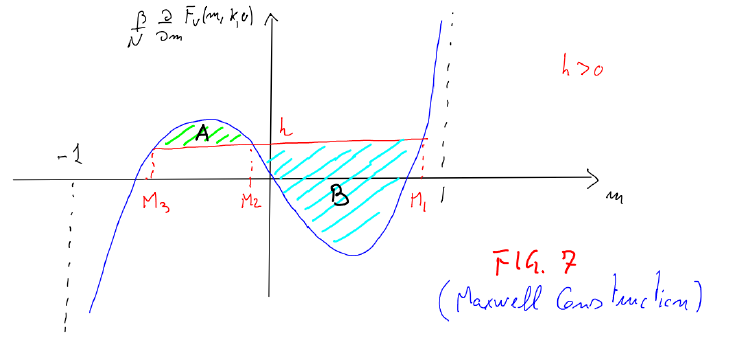
\includegraphics[width=0.9\textwidth]{variational_energy_h.png}
    \caption{} %TODO CAPTION
    \label{fig:variational_energy_h}
\end{figure}

To simplify notation, let's denote as $f_i$ the free variational energy evaluated at a solution $M_i$:
\begin{align*}
    f_i = \frac{\beta F_V(M_i, K, h)}{N} = \frac{\beta F_V(M_i, K, 0)}{N} - hM_i  
\end{align*}
Then note that differences of $f_i$ can be rewritten as integrals, which can be roughly evaluated by looking at fig. \ref{fig:variational_energy_h}. Then, for $h > 0$:
\begin{align*}
    f_1 - f_2 &= \int_{M_2}^{M_1} \left(\frac{\beta}{N} \pdv{m} F_V(m, K, 0) - h\right) \dd{m} = -\text{\textcolor{Blue}{Area of \textbf{B}}} < 0 \Rightarrow f_1 < f_2\\
    f_2 - f_3 &= \int_{M_3}^{M_2} \left(\frac{\beta}{N} \pdv{m} F_V(m, K, 0) - h\right) \dd{m} = -\text{\textcolor{PineGreen}{Area of \textbf{A}}} < 0 \Rightarrow f_2 < f_3\\
    f_1-f_3 &= \int_{M_3}^{M_1} \left(\frac{\beta}{N} \pdv{m} F_V(m, K, 0) - h\right) \dd{m} = \text{\textcolor{PineGreen}{Area of \textbf{A}}}-\text{\textcolor{Blue}{Area of \textbf{B}}} < 0 \Rightarrow f_1 < f_3\\
\end{align*}
Summarizing:
\begin{enumerate}
    \item For $h > 0$, the area of \textbf{\textcolor{Blue}{B}} is always bigger than that of \textbf{\textcolor{PineGreen}{A}}. So, at the end, $f_1 < f_2 < f_3$.
    \item For $h = 0$, the two areas \textbf{\textcolor{PineGreen}{A}} and \textbf{\textcolor{Blue}{B}} become equal, and $f_1$ and $f_3$ are two degenerate minima. 
    \item On the other hand, if $h < 0$, all inequalities are reversed, and $f_3 < f_2 < f_1$. So, when $h$ changes sign, the system \textit{jumps} to a different minimum. 
\end{enumerate}

Intuitively, a $h > 0$ leads to a \textit{preference} for a positive magnetization, and, conversely, $h < 0$ for a negative magnetization. 

\medskip

A plot of the solution $M(K,h)$ corresponding to the minimum of $F_V$ as a function of $h$ is shown in fig. \ref{fig:Mhplot}.

\begin{figure}[H]
    \centering
    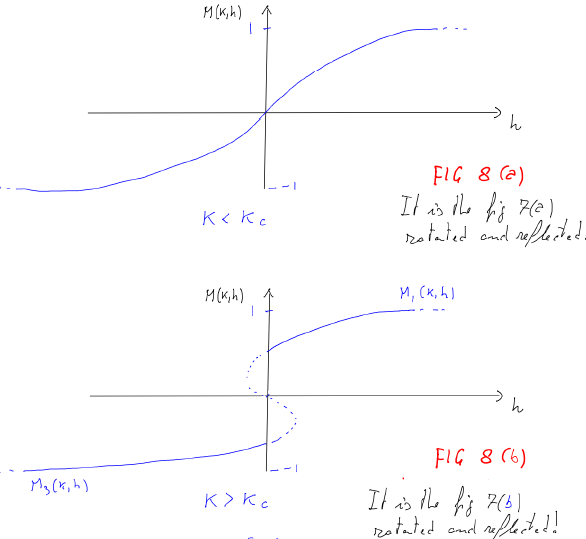
\includegraphics[width=0.8\textwidth]{Mhplot.png}
    \caption{
    Plot of $M(K,h)$ (variational estimate of magnetization, obtained by minimizing $F_V$) as a function of the external field $h$, which can be obtained by rotating and reflecting fig. \ref{fig:hplot}.    
    If $K < K_c$ (top) the magnetization varies continuously as a function of $h$. If $K > K_c$, instead, (bottom) there is a discontinuity at $h=0$, given by the system's transition to a different minimum ($M_3$ instead of $M_1$)}
    \label{fig:Mhplot}
\end{figure}

All of these results about criticality are summarized in fig. \ref{fig:phase-diagram-uniform}.

\begin{figure}[H]
    \centering
    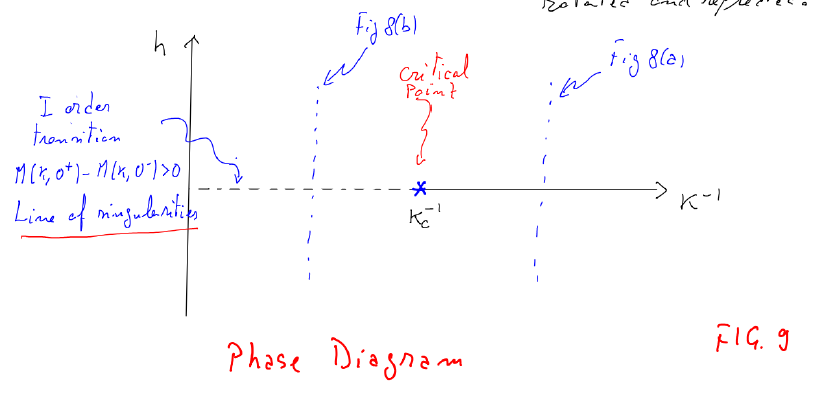
\includegraphics[width=0.9\textwidth]{phase-diagram-uniform.png}
    \caption{Phase diagram representing all the singular points of $M(K,h)$ as a dashed line. Any curve surpassing the dashed part (left of $K_c^{-1}$) has a discontinuity (first-order transition). One such path is the one in the bottom plot of fig. \ref{fig:Mhplot}. On the other hand, a curve surpassing $h=0$ \textit{at the right} of $K_c^{-1}$, however, is smooth; and one such example is given by the top curve of fig. \ref{fig:Mhplot}. So, starting at a point $(h, K^{-1})$ with $h>0$, we can construct \textit{two kinds} of paths arriving to the phase with $h < 0$: one passing through a high-temperature state and without phase-transitions, and one with a phase-transition at a low temperature.
    Something analogous happens for the vapour-liquid transition: it can be observed as an abrupt change (phase transition) at sufficiently low temperatures, or as a completely smooth process if pressure is increased such that phase differences are removed (the \q{gas looks like a liquid}).}
    \label{fig:phase-diagram-uniform}
\end{figure}

We conclude by stressing that the \textbf{singularities} at $h=0$ and $K > K_c$ \textit{emerge} from to the variational principle as a consequence of the minimization.  

\begin{appr}\textbf{Remarks on the mean-field approximation}. The Mean Field (MF) model predicts a phase transition in all $d > 0$. However we know that this is not true in $d=1$, where no phase transition is observed (pag. \pageref{par:no-phase-transition}). Still, for $d > 1$ the MF is at least qualitatively correct. Impressively, such a simple model agrees \textit{exactly} with simulation at $d \geq 4$, at least for the behaviour of magnetization near criticality. 
\end{appr}

\begin{appr}\textbf{Mean Field and symmetry breaking}. For $h=0$, the Ising Model Hamiltonian:
    \begin{align*}
        \mathcal{H}(\bm{\sigma}) = -J \sum_{\langle x,y \rangle} \sigma_x \sigma_y
    \end{align*} 
    is \textbf{symmetric} with respect to the transformation $\sigma_x \to -\sigma_x$ $\forall x$, i.e. $\mathcal{H}(\bm{\sigma}) = -\mathcal{H}(\bm{\sigma})$. In any \textbf{finite} system ($N < \infty$), this symmetry implies that $\langle \sigma_x \rangle = - \langle \sigma_x \rangle \Rightarrow \langle \sigma_x \rangle = 0$, meaning that no spontaneous magnetization can be observed. However, in the \textbf{infinite volume}, this symmetry is \textbf{spontaneously broken} below some critical temperature and $\langle \sigma_x \rangle \neq 0$. %TODO Add reference to pag. 13 ch. 6 of the notes (?)
    
    We have shown how this occurs in the mean field approximation. Specifically, the symmetry that is broken for the Ising model is $\mathbb{Z}_2$.
    
    \medskip

    If we instead consider the Hamiltonian:
    \begin{align*}
        H(\bm{\sigma}) = -J \sum_{\langle x,y \rangle} \bm{\sigma_x} \cdot \bm{\sigma_y}
    \end{align*}
    where $\bm{\sigma_x} \in \mathbb{R}^n$ and $\norm{\bm{\sigma_x}} = 1$, then the group symmetry is $\mathrm{O}(n)$, the orthogonal group, and $H(R \bm{\sigma}) = H(\bm{\sigma})$, where $R$ is a $n\times n$ matrix such that $\norm{R \bm{\sigma}} = \norm{\bm{\sigma}}^2 = 1$, i.e. a orthogonal (\q{rotation}) matrix satisfying $R^TR = RR^T = \mathbb{I}$. 

    There are rigorous results establishing that discrete symmetries like $\mathbb{Z}_2$ cannot be spontaneously broken in $d=1$ (Landau arguments) whereas continuous symmetries, like $\mathrm{O}(n)$, cannot be spontaneously broken in $d \leq 2$ (Mermin-Wagner theorem). In both cases only short-range interactions are assumed.
\end{appr}




\end{document}
